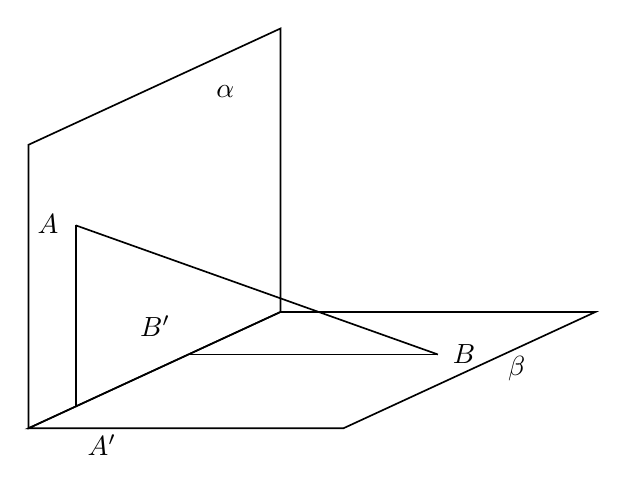
\begin{tikzpicture}[x=1cm,y=1cm,line width=.6pt,font=\normalsize,
  geometry edge/.style={solid,line width=.6pt},
  geometry label/.style={font=\normalsize,inner sep=2pt}]
% Plane alpha (left, vertical) meets plane beta (bottom) along line l.
% A in alpha, A' foot on l, AA' drawn. B in beta, B' foot on l, B'B drawn.
% A'=(0,0); l runs from A' to P0=(2.6,1.2).
\coordinate (Apr) at (0,0);
\coordinate (P0) at (2.6,1.2);
\coordinate (Talpha) at (2.6,4.8);
\coordinate (TLalpha) at (-0.6,3.323076923);
\coordinate (Rbeta) at (6.6,1.2);
\coordinate (R2beta) at (3.4,-0.276923077);
\coordinate (L2beta) at (-0.6,-0.276923077);
\coordinate (A) at (0,2.3);
\coordinate (Bp) at (1.43,0.66);
\coordinate (B) at (4.6,0.66);
% Plane outlines (solid)
\draw[geometry edge] (L2beta)--(P0)--(Talpha)--(TLalpha)--cycle;
\draw[geometry edge] (L2beta)--(P0)--(Rbeta)--(R2beta)--cycle;
% Interior segments
\draw[geometry edge] (A)--(Apr);
\draw[geometry edge] (A)--(B);
\draw[geometry edge] (Bp)--(B);
% Labels placed clear of all strokes
\node[geometry label,anchor=east] at (-0.14,2.32) {$A$};
\node[geometry label,below right=2pt,xshift=0.00bp,yshift=-6.00bp] at (Apr) {$A'$};
\node[geometry label,anchor=east] at (1.28,1.02) {$B'$};
\node[geometry label,anchor=west,xshift=-2.00bp,yshift=0.00bp] at (4.78,.66) {$B$};
\node[geometry label,anchor=center] at (1.9,4.0) {$\alpha$};
\node[geometry label,anchor=center,xshift=0.00bp,yshift=-2.00bp] at (5.6,0.55) {$\beta$};
\end{tikzpicture}
